\subsection{Исходные изображения}
Выберем изображения, которые содержат прямые линии. Первым изображением будет логотип нашего любимого университета:
\begin{figure}[ht!]
    \centering
    
\includegraphics[width=0.55\textwidth]{images/lines/source/ITMO_LOGO.jpeg}
    \caption{Логотип университета ИТМО}
    \label{img:src_logo}
\end{figure} 

Также возьмём рисунок, составленный из прямых линий:

\begin{figure}[ht!]
    \centering
    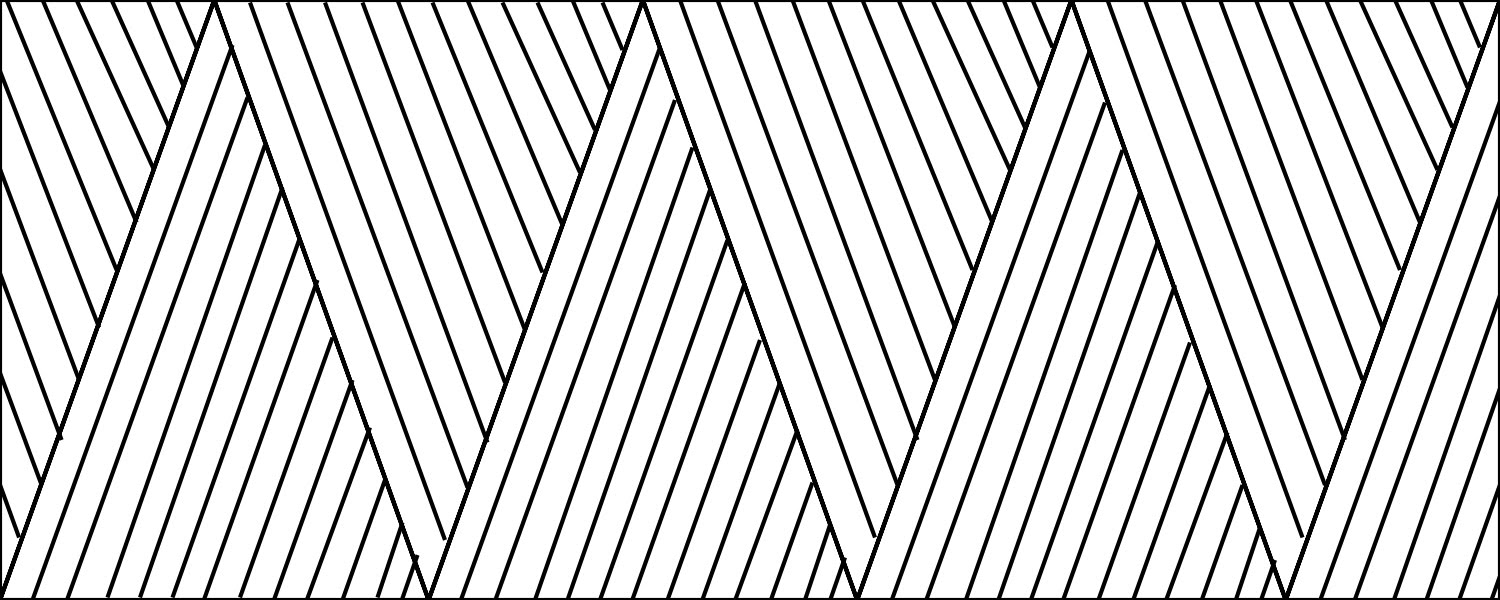
\includegraphics[width=0.55\textwidth]{images/lines/source/wovenlinesfinal.jpeg}
    \caption{Паркет ёлочкой}
    \label{img:src_fir}
\end{figure} 

И обратимся к творчеству абстракциониста Пита Мондриана:

\begin{figure}[ht!]
    \centering
    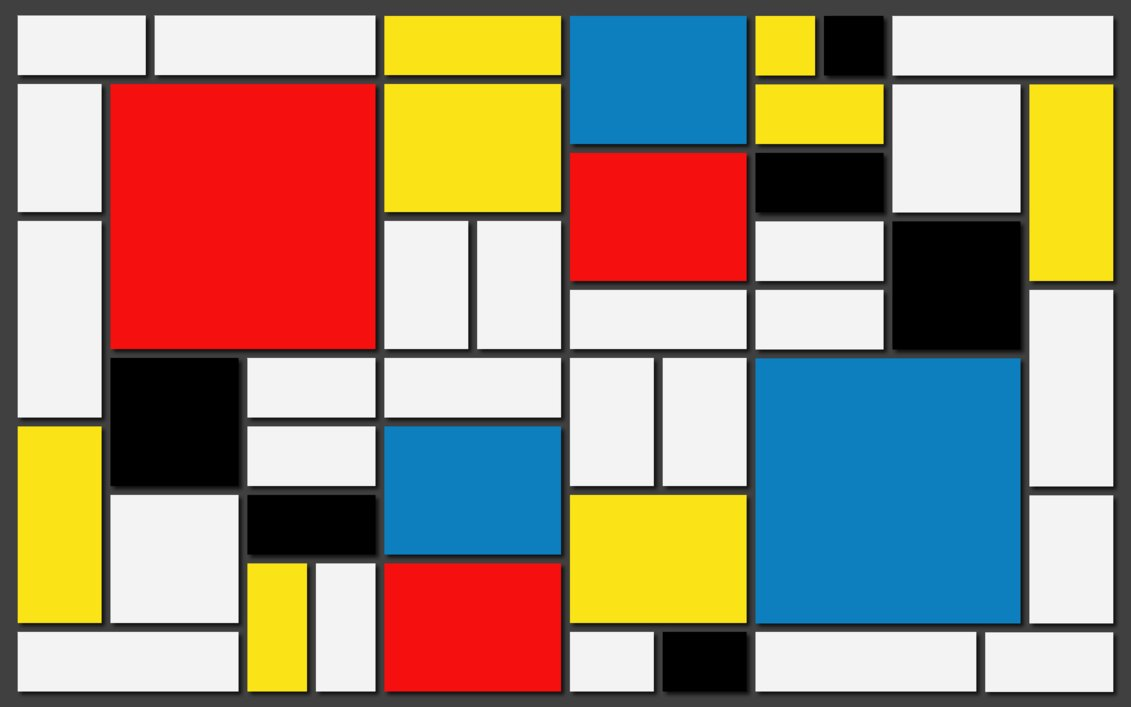
\includegraphics[width=0.55\textwidth]{images/lines/source/Piet_Mondriaan_-_03.jpg}
    \caption{Цифровая репродукция картины Пита Мондриана}
    \label{img:src_piet}
\end{figure} 

\subsection{Программа на языке Python}
\begin{lstlisting}[caption={Исходный код функции для нахождения и отображения прямых линий с помощью преобразования Хафа}, label={lst:line_compute}]
    def line_detection(option, image):
        # Grayscale image
        # edged = cv.cvtColor(image, cv.COLOR_BGR2GRAY)
        # Canny edges
        edged = cv.Canny(image, 250, 270, None, 3)
        match option:
            case 0:
                # output of the original image
                cv.imshow('Source Image', image)
                cv.waitKey(0)
            case 1:
                # Hough transform
                # creating image copies
                result = image.copy()
                result_p = image.copy()
                # computing lines via classic Hough transform
                lines = cv.HoughLines(edged, 1, np.pi / 180, 150)
                # computing lines via probabilistic Hough transform
                lines_p = cv.HoughLinesP(edged, 1, np.pi / 180, 50, None, 30, 4)
                #
                angles = np.linspace(-np.pi / 2, np.pi / 2, 360, endpoint=False)
                # Accumulator computing
                ah, _, _ = skimage.transform.hough_line(edged, theta=angles)
                mx = 0
                mn = 10000
                for i in range(len(lines_p)):
                    # overlaying lines found by using probabilistic transform and their edges
                    line = lines_p[i][0]
                    pt1 = (line[0], line[1])
                    pt2 = (line[2], line[3])
                    cv.line(result_p, pt1, pt2, (0, 255, 255), 5, cv.LINE_AA)
                    cv.circle(result_p, pt1, 5, (0, 0, 255), -1)
                    cv.circle(result_p, pt2, 5, (0, 0, 255), -1)
                    # computing the shortest and longest lines
                    norm = np.linalg.norm(np.array(pt2) - np.array(pt1))
                    if norm < mn:
                        mn = round(norm, 2)
                    if norm > mx:
                        mx = round(norm, 2)
                for j in range(len(lines)):
                    # overlaying lines found by using classic transform and their edges
                    rho = lines[j][0][0]
                    theta = lines[j][0][1]
                    a, b = math.cos(theta), math.sin(theta)
                    x0, y0 = a * rho, b * rho
                    pt1 = (np.int32(x0 + 1000 * (-b)), np.int32(y0 + 1000 * a))
                    pt2 = (np.int32(x0 - 1000 * (-b)), np.int32(y0 - 1000 * a))
                    cv.line(result, pt1, pt2, (0, 255, 255), 5, cv.LINE_AA)
                    cv.circle(result, pt1, 5, (255, 0, 0), -1)
                    cv.circle(result, pt2, 5, (255, 0, 0), -1)
                # cv.imwrite('results/lines/Klinom_p.jpg', result_p)
                # transferring recieved images and data to function of creating a comparative image
                image_displaying(image, edged, result_p, result, ah, mn, mx, len(lines_p))
                case _:
                    print('Wrong option! Enter the right number')
    \end{lstlisting}

    \begin{lstlisting}[caption={Исходный код функции для создания сравнительного изображения с результатами преобразования}, label={lst:show_images}]
    def image_displaying(source, canny, finale_p, finale, parametric, mn, mx, nmbr):
        # creating figure with mosaic layout
        fig,  axs = plt.subplot_mosaic([['src', 'can'], ['fin', 'finp'], ['p', 'info']], layout='tight', figsize=(9.2, 7.8))
        # plotting images
        axs['src'].imshow(cv.cvtColor(source, cv.COLOR_BGR2RGB))
        axs['can'].imshow(canny, cmap=matplotlib.cm.gray)
        axs['fin'].imshow(cv.cvtColor(finale, cv.COLOR_BGR2RGB))
        axs['finp'].imshow(cv.cvtColor(finale_p, cv.COLOR_BGR2RGB))
        axs['p'].imshow(cv.resize(parametric.astype(np.float32) / np.max(parametric),
                                (parametric.shape[1], 300)), cmap=matplotlib.cm.gray)
        # turning off axes
        axs['src'].axis('off')
        axs['can'].axis('off')
        axs['fin'].axis('off')
        axs['finp'].axis('off')
        axs['p'].axis('off')
        axs['info'].axis('off')
        axs['src'].set_title('Image')
        axs['can'].set_title('Canny edges')
        axs['fin'].set_title('Hough')
        axs['finp'].set_title('Probabilistic Hough')
        axs['p'].set_title('Parameter space')
        # plotting number of lines found, minimum amd maximum length
        axs['info'].text(0.5, 0.5, f'Number of lines: {nmbr}\nShortest line: {mn}\nLongest line: {mx}', size=25,
                        ha='center',
                        va='center',
                        bbox=dict(boxstyle="square",
                                ec=(1., 0.5, 0.5),
                                fc=(1., 0.8, 0.8)
                                )
                        )
        # displaying and saving the plot
        plt.show()
        fig.savefig('results/lines/ITMO.jpg')
        plt.close()
        \end{lstlisting}


\subsection{Результаты преобразования}

\begin{figure}[ht!]
    \centering
    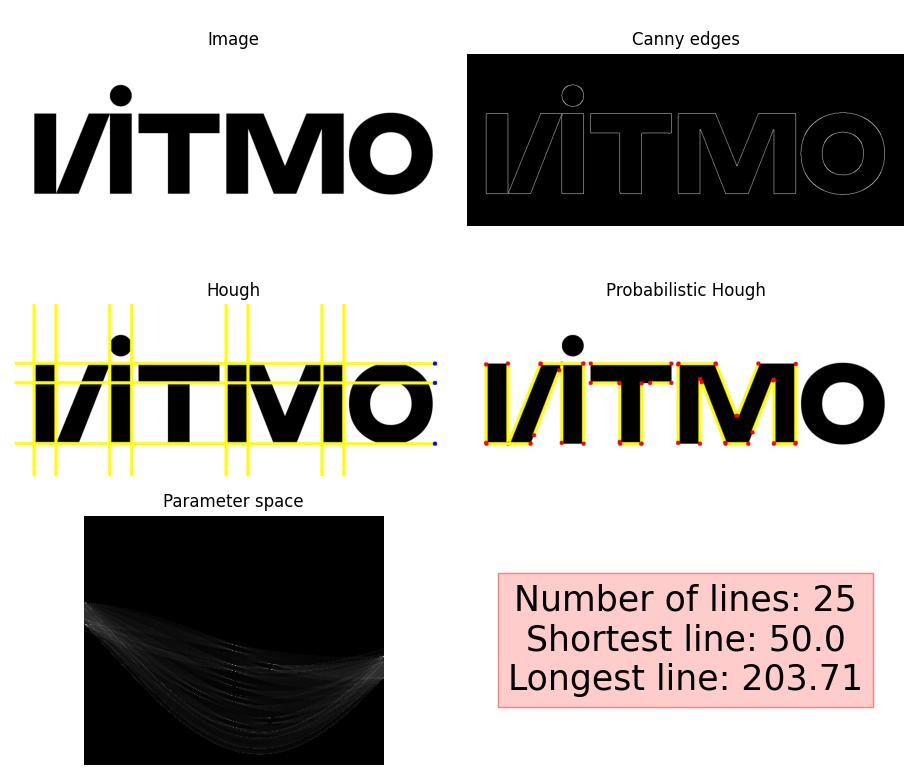
\includegraphics[width=\textwidth]{images/lines/ITMO.jpg}
    \caption{Исходное изображение 1; контуры изображения, полученные алгоритмом Кэнни; результаты классического и вероятностного преобразованием Хафа; пространство параметров;подсчёт прямых}
    \label{img:fin_ITMO}
\end{figure} 

\clearpage

Вероятностное преобразование Хафа в результате работы выдаёт значения крайних точек распознанных линий, поэтому результат его работы позволяет довольно точно выделить их. Классическое преобразование, в свою очередь, возвращает угол наклона и длину радиус вектора прямой, которой принадлежит исходная линия. Наши выводы подтверждаются рисунками \ref*{img:fin_ITMO}, \ref*{img:src_fir} и \ref*{img:fin_piet}.

\begin{figure}[ht!]
    \centering
    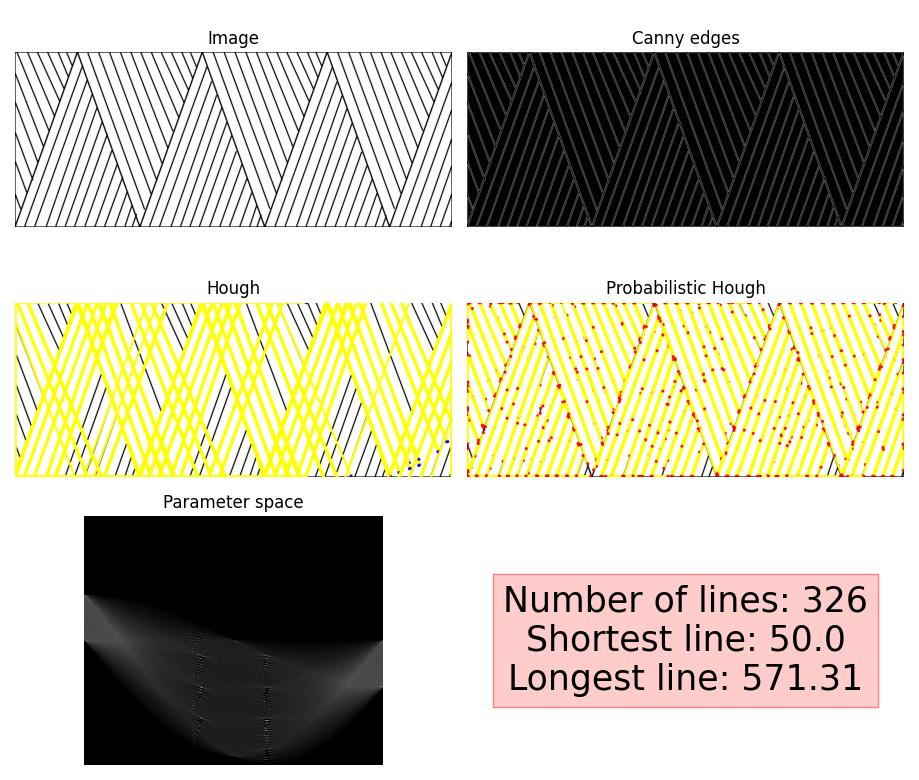
\includegraphics[width=\textwidth]{images/lines/simple_lines.jpg}
    \caption{Исходное изображение 2; контуры изображения, полученные алгоритмом Кэнни; результаты классического и вероятностного преобразованием Хафа; пространство параметров;подсчёт прямых}
    \label{img:fin_fir}
\end{figure}

\begin{figure}[ht!]
    \centering
    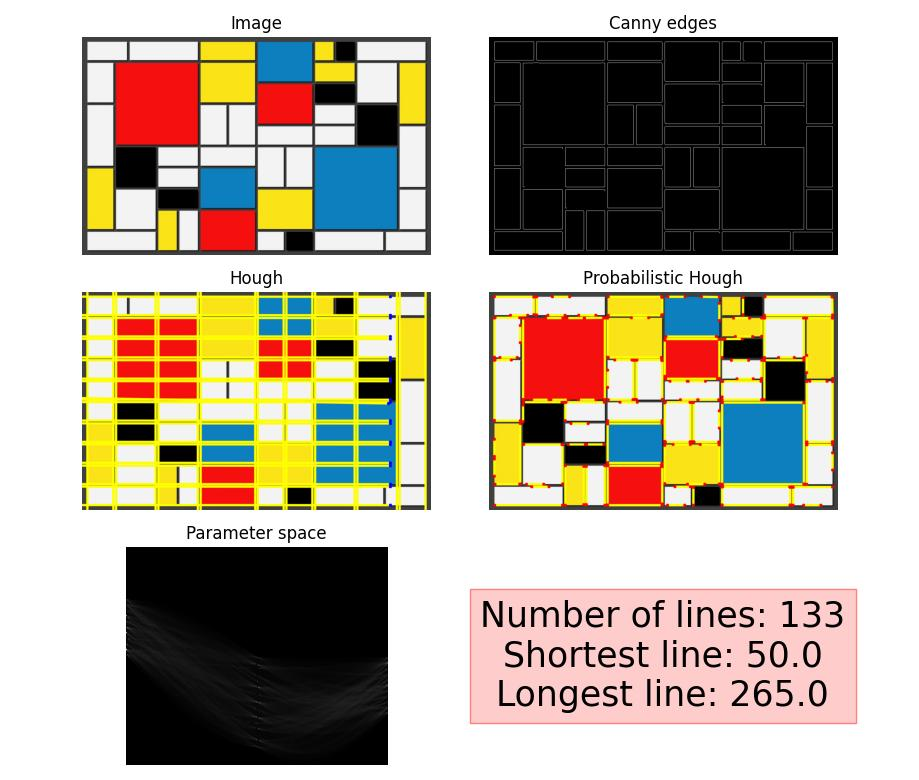
\includegraphics[width=\textwidth]{images/lines/Mondrian_03.jpg}
    \caption{Исходное изображение 3; контуры изображения, полученные алгоритмом Кэнни; результаты классического и вероятностного преобразованием Хафа; пространство параметров;подсчёт прямых}
    \label{img:fin_piet}
\end{figure}

\clearpage
% \subsection{Бонус. Клином красным бей белых!}

Теперь попробуем применить преобразование к полутоновым изображениям:

\begin{figure}[ht!]
    \centering
    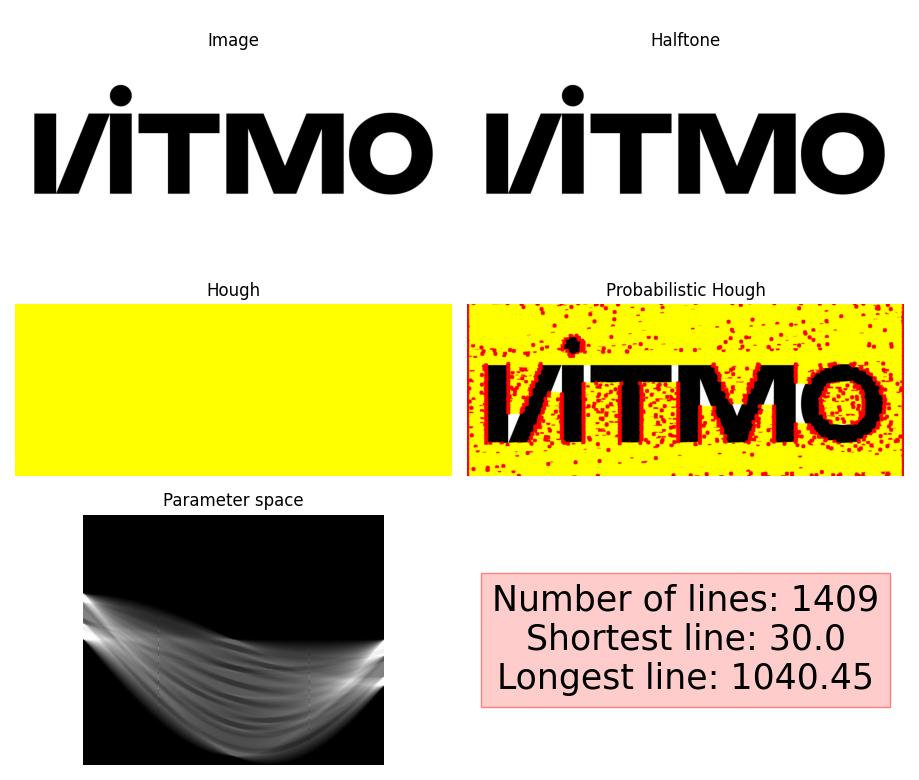
\includegraphics[width=\textwidth]{images/lines/ITMO_gray.jpg}
    \caption{Исходное изображение 1; полутоновое изображение; результаты классического и вероятностного преобразованием Хафа; пространство параметров;подсчёт прямых}
    \label{img:fin_ITMO_gray}
\end{figure} 

Можно констатировать, что в данном случае преобразование Хафа не справляется с поставленной задачей. Это связано с тем, что алгоритм воспринимает в качестве контуров всю область изображения вокруг чёрных участков. Поэтому на изображении с логотипом прямыми линиями были выделена вся область вокруг букв (см. рисунок \ref*{img:fin_ITMO_gray}), исключение составили участки, ширина которых составляла менее 30 пикселей. Аналогичный результат получился в случае обработке репродукции Пита Мондриана (см. рисунок \ref*{img:fin_piet_gray}).

Из-за тонких чёрных линий 2 изображения (рисунок \ref{img:src_fir}) линии полностью покрыли его, в результате чего мы получили жёлтый прямоугольник (см. рисунок \ref*{img:fin_fir_gray}).

\begin{figure}[ht!]
    \centering
    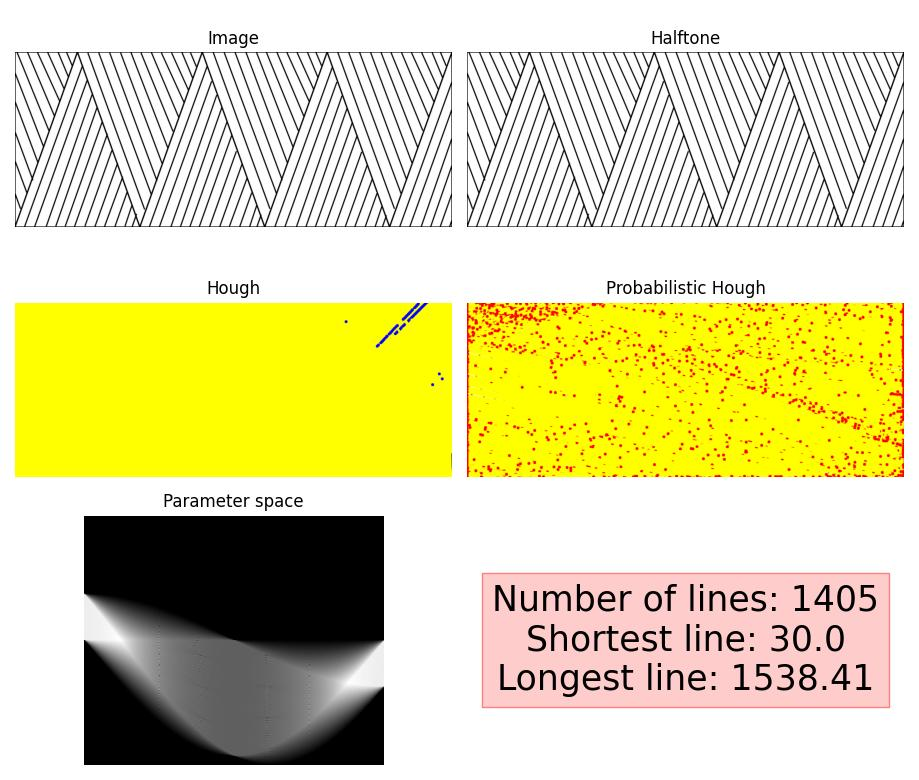
\includegraphics[width=\textwidth]{images/lines/simple_lines_gray.jpg}
    \caption{Исходное изображение 2; полутоновое изображение; результаты классического и вероятностного преобразованием Хафа; пространство параметров;подсчёт прямых}
    \label{img:fin_fir_gray}
\end{figure}

\begin{figure}[ht!]
    \centering
    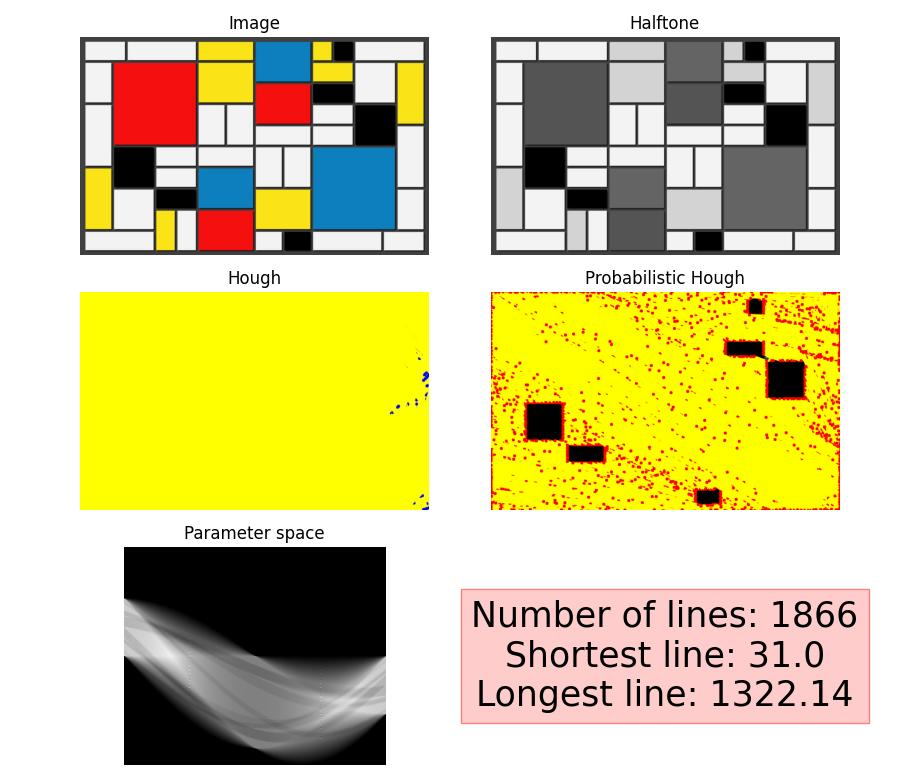
\includegraphics[width=\textwidth]{images/lines/Mondrian_03_gray.jpg}
    \caption{Исходное изображение 3; полутоновое изображение; результаты классического и вероятностного преобразованием Хафа; пространство параметров;подсчёт прямых}
    \label{img:fin_piet_gray}
\end{figure}

\clearpage